\documentclass[8pt,aspectratio=169]{beamer}
\usetheme{Madrid}
\usepackage{graphicx}
\usepackage{booktabs}
\usepackage{adjustbox}
\usepackage{multicol}
\usepackage{amsmath}
\usepackage{amssymb}
\usepackage{listings}
\usepackage{xcolor}

% Color definitions
\definecolor{mlblue}{RGB}{0,102,204}
\definecolor{mlpurple}{RGB}{51,51,178}
\definecolor{mllavender}{RGB}{173,173,224}
\definecolor{mllavender2}{RGB}{193,193,232}
\definecolor{mllavender3}{RGB}{204,204,235}
\definecolor{mllavender4}{RGB}{214,214,239}
\definecolor{mlorange}{RGB}{255, 127, 14}
\definecolor{mlgreen}{RGB}{44, 160, 44}
\definecolor{mlred}{RGB}{214, 39, 40}
\definecolor{mlgray}{RGB}{127, 127, 127}

% Additional colors for template compatibility
\definecolor{lightgray}{RGB}{240, 240, 240}
\definecolor{midgray}{RGB}{180, 180, 180}

% Solidity colors
\definecolor{solkeyword}{RGB}{0,102,153}
\definecolor{solstring}{RGB}{163,21,21}
\definecolor{solcomment}{RGB}{0,128,0}
\definecolor{solnumber}{RGB}{0,128,128}

% Solidity language definition
\lstdefinelanguage{Solidity}{
  keywords={pragma, solidity, contract, function, public, private, external, internal, view, pure, payable, returns, return, if, else, for, while, mapping, address, uint, uint256, int, string, bool, bytes, bytes32, event, emit, modifier, require, constructor, memory, storage, calldata, msg, sender, value, this, new, delete, true, false},
  keywordstyle=\color{solkeyword}\bfseries,
  sensitive=true,
  comment=[l]{//},
  morecomment=[s]{/*}{*/},
  commentstyle=\color{solcomment}\ttfamily,
  stringstyle=\color{solstring}\ttfamily,
  morestring=[b]',
  morestring=[b]"
}

% Apply custom colors to Madrid theme
\setbeamercolor{palette primary}{bg=mllavender3,fg=mlpurple}
\setbeamercolor{palette secondary}{bg=mllavender2,fg=mlpurple}
\setbeamercolor{palette tertiary}{bg=mllavender,fg=white}
\setbeamercolor{palette quaternary}{bg=mlpurple,fg=white}
\setbeamercolor{structure}{fg=mlpurple}
\setbeamercolor{section in toc}{fg=mlpurple}
\setbeamercolor{subsection in toc}{fg=mlblue}
\setbeamercolor{title}{fg=mlpurple}
\setbeamercolor{frametitle}{fg=mlpurple,bg=mllavender3}
\setbeamercolor{block title}{bg=mllavender2,fg=mlpurple}
\setbeamercolor{block body}{bg=mllavender4,fg=black}

\setbeamertemplate{navigation symbols}{}
\setbeamertemplate{itemize items}[circle]
\setbeamertemplate{enumerate items}[default]
\setbeamersize{text margin left=5mm,text margin right=5mm}

\newcommand{\bottomnote}[1]{%
\vfill
\vspace{-2mm}
\textcolor{mllavender2}{\rule{\textwidth}{0.4pt}}
\vspace{1mm}
\footnotesize
\textbf{#1}
}

% TikZ and pgfplots packages
\usepackage{tikz}
\usepackage{pgfplots}
\pgfplotsset{compat=1.18}
\usetikzlibrary{arrows.meta, positioning, shapes.geometric, shapes.symbols, calc, decorations.pathmorphing, mindmap}

\title{Stablecoins \& CBDCs: A Visual Introduction}
\subtitle{Standalone Mini-Lecture}
\author{Prof.~Dr.~Joerg Osterrieder}
\institute{University Lecture Series}
\date{\today}
\begin{document}

% ==================== FRAME 1: TITLE ====================
\begin{frame}[plain]
\vspace{2cm}
\begin{center}
{\Huge\color{mlpurple} Stablecoins \& CBDCs: A Visual Introduction}\\[0.4cm]
{\Large\color{mlblue} Standalone Mini-Lecture}\\[0.3cm]
\textcolor{mlgray}{\rule{6cm}{0.4pt}}\\[0.3cm]
{\small\itshape ``In the world of crypto, stability is the hardest trick to pull off''}\\[1.5cm]
{\normalsize Prof.~Dr.~Joerg Osterrieder}\\[0.2cm]
{\small University Lecture Series}\\[0.2cm]
{\small \today}
\end{center}
\end{frame}

% ==================== FRAME 2: THE PRICE STABILITY PROBLEM ====================
\begin{frame}{The Price Stability Problem}
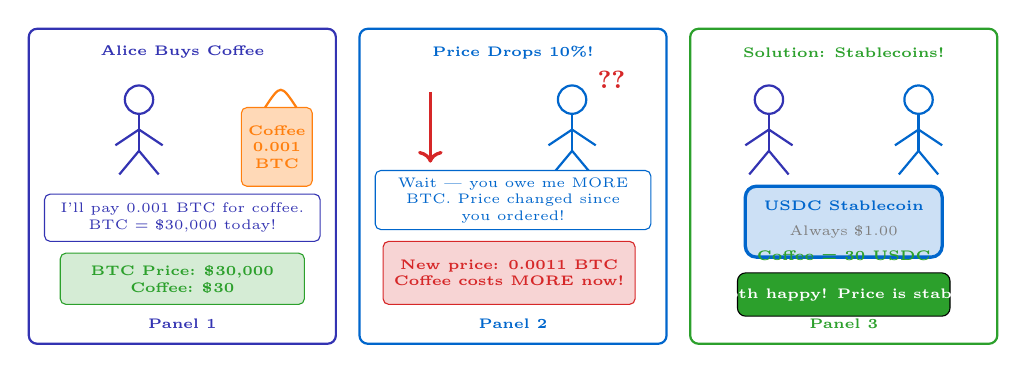
\begin{tikzpicture}
  % Panel borders
  \draw[thick, mlpurple, rounded corners=3pt] (0.1,0.2) rectangle (4.0,4.2);
  \draw[thick, mlblue,   rounded corners=3pt] (4.3,0.2) rectangle (8.2,4.2);
  \draw[thick, mlgreen,  rounded corners=3pt] (8.5,0.2) rectangle (12.4,4.2);

  % --- Panel 1: Alice wants coffee with Bitcoin ---
  \node[font=\tiny\bfseries, mlpurple] at (2.05,3.9) {Alice Buys Coffee};
  % Coffee cup
  \draw[fill=mlorange!30, draw=mlorange, rounded corners=2pt] (2.8,2.2) rectangle (3.7,3.2);
  \draw[mlorange, thick] (3.1,3.2) .. controls (3.3,3.5) .. (3.5,3.2);
  \node[font=\tiny\bfseries, mlorange, align=center] at (3.25,2.7) {Coffee\\0.001\\BTC};
  % Alice stick figure
  \draw[mlpurple,thick] (1.5,3.3) circle (0.18);
  \draw[mlpurple,thick] (1.5,3.12) -- (1.5,2.65);
  \draw[mlpurple,thick] (1.5,2.92) -- (1.2,2.72);
  \draw[mlpurple,thick] (1.5,2.92) -- (1.8,2.72);
  \draw[mlpurple,thick] (1.5,2.65) -- (1.25,2.35);
  \draw[mlpurple,thick] (1.5,2.65) -- (1.75,2.35);
  % Speech bubble
  \draw[fill=white, draw=mlpurple, rounded corners=2pt] (0.3,1.5) rectangle (3.8,2.1);
  \node[font=\tiny, mlpurple, align=center] at (2.05,1.8) {I'll pay 0.001 BTC for coffee.\\BTC = \$30{,}000 today!};
  % BTC price indicator
  \draw[fill=mlgreen!20, draw=mlgreen, rounded corners=2pt] (0.5,0.7) rectangle (3.6,1.35);
  \node[font=\tiny\bfseries, mlgreen, align=center] at (2.05,1.02) {BTC Price: \$30{,}000\\Coffee: \$30};
  \node[font=\tiny\bfseries, mlpurple] at (2.05,0.45) {Panel 1};

  % --- Panel 2: BTC dropped 10%, Bob confused ---
  \node[font=\tiny\bfseries, mlblue] at (6.25,3.9) {Price Drops 10\%!};
  % Bob stick figure (barista, confused)
  \draw[mlblue,thick] (7.0,3.3) circle (0.18);
  \draw[mlblue,thick] (7.0,3.12) -- (7.0,2.65);
  \draw[mlblue,thick] (7.0,2.92) -- (6.7,2.72);
  \draw[mlblue,thick] (7.0,2.92) -- (7.3,2.72);
  \draw[mlblue,thick] (7.0,2.65) -- (6.75,2.35);
  \draw[mlblue,thick] (7.0,2.65) -- (7.25,2.35);
  % Question marks above Bob
  \node[font=\small\bfseries, mlred] at (7.5,3.55) {??};
  % Down arrow for price
  \draw[->, very thick, mlred] (5.2,3.4) -- (5.2,2.5);
  \node[font=\tiny\bfseries, mlred, align=center] at (5.2,2.2) {BTC now\\-10\%};
  % New bill
  \draw[fill=mlred!20, draw=mlred, rounded corners=2pt] (4.6,0.7) rectangle (7.8,1.5);
  \node[font=\tiny\bfseries, mlred, align=center] at (6.2,1.1) {New price: 0.0011 BTC\\Coffee costs MORE now!};
  % Speech bubble from Bob
  \draw[fill=white, draw=mlblue, rounded corners=2pt] (4.5,1.65) rectangle (8.0,2.4);
  \node[font=\tiny, mlblue, align=center] at (6.25,2.02) {Wait --- you owe me MORE\\BTC. Price changed since\\you ordered!};
  \node[font=\tiny\bfseries, mlblue] at (6.25,0.45) {Panel 2};

  % --- Panel 3: Solution - stablecoins ---
  \node[font=\tiny\bfseries, mlgreen] at (10.45,3.9) {Solution: Stablecoins!};
  % Alice happy stick figure
  \draw[mlpurple,thick] (9.5,3.3) circle (0.18);
  \draw[mlpurple,thick] (9.5,3.12) -- (9.5,2.65);
  \draw[mlpurple,thick] (9.5,2.92) -- (9.2,2.72);
  \draw[mlpurple,thick] (9.5,2.92) -- (9.8,2.72);
  \draw[mlpurple,thick] (9.5,2.65) -- (9.25,2.35);
  \draw[mlpurple,thick] (9.5,2.65) -- (9.75,2.35);
  % Bob happy stick figure
  \draw[mlblue,thick] (11.4,3.3) circle (0.18);
  \draw[mlblue,thick] (11.4,3.12) -- (11.4,2.65);
  \draw[mlblue,thick] (11.4,2.92) -- (11.1,2.72);
  \draw[mlblue,thick] (11.4,2.92) -- (11.7,2.72);
  \draw[mlblue,thick] (11.4,2.65) -- (11.15,2.35);
  \draw[mlblue,thick] (11.4,2.65) -- (11.65,2.35);
  % USDC token badge
  \draw[fill=mlblue!20, draw=mlblue, very thick, rounded corners=4pt]
       (9.2,1.3) rectangle (11.7,2.2);
  \node[font=\tiny\bfseries, mlblue, align=center] at (10.45,1.95) {USDC Stablecoin};
  \node[font=\tiny, mlgray, align=center] at (10.45,1.62) {Always \$1.00};
  \node[font=\tiny\bfseries, mlgreen, align=center] at (10.45,1.32) {Coffee = 30 USDC};
  % Green badge
  \draw[fill=mlgreen, rounded corners=3pt] (9.1,0.55) rectangle (11.8,1.1);
  \node[font=\tiny\bfseries, white, align=center] at (10.45,0.82) {Both happy! Price is stable!};
  \node[font=\tiny\bfseries, mlgreen] at (10.45,0.45) {Panel 3};
\end{tikzpicture}

\bottomnote{Stablecoins solve the volatility problem: 1 USDC always equals \$1 regardless of crypto market swings.}
\end{frame}

% ==================== FRAME 3: WHAT IS A STABLECOIN? ====================
\begin{frame}{What is a Stablecoin?}
\begin{columns}[c]
  \begin{column}{0.46\textwidth}
    \centering
    {\small\bfseries\color{mlred} Volatile Crypto (BTC / ETH)}\\[0.2cm]
    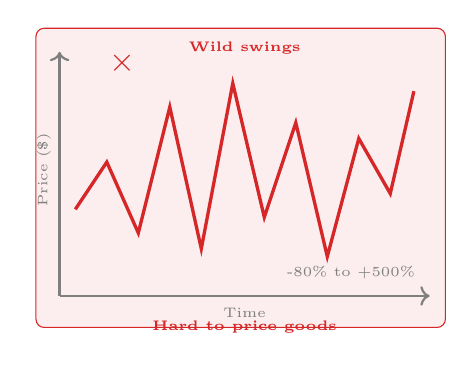
\begin{tikzpicture}
      % Price chart background
      \draw[fill=mlred!8, draw=mlred, rounded corners=3pt] (0,0) rectangle (5.2,3.8);
      % Axes
      \draw[->, mlgray, thick] (0.3,0.4) -- (5.0,0.4);
      \draw[->, mlgray, thick] (0.3,0.4) -- (0.3,3.5);
      \node[font=\tiny, mlgray, rotate=90] at (0.1,2.0) {Price (\$)};
      \node[font=\tiny, mlgray] at (2.65,0.18) {Time};
      % Volatile price line
      \draw[mlred, very thick]
        (0.5,1.5) -- (0.9,2.1) -- (1.3,1.2) -- (1.7,2.8) -- (2.1,1.0) --
        (2.5,3.1) -- (2.9,1.4) -- (3.3,2.6) -- (3.7,0.9) -- (4.1,2.4) --
        (4.5,1.7) -- (4.8,3.0);
      % Labels
      \node[font=\tiny\bfseries, mlred, align=center] at (2.65,3.55) {Wild swings};
      \node[font=\tiny, mlgray, align=center] at (4.0,0.7) {-80\% to +500\%};
      % Unhappy face
      \node[font=\large, mlred] at (1.1,3.35) {$\times$};
      \node[font=\tiny\bfseries, mlred, align=center] at (2.65,0.0) {Hard to price goods};
    \end{tikzpicture}
  \end{column}

  \begin{column}{0.08\textwidth}
    \centering
    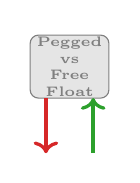
\begin{tikzpicture}
      \draw[fill=mlgray!20, draw=mlgray, rounded corners=3pt]
            (-0.3,1.5) rectangle (0.7,2.3);
      \node[font=\tiny\bfseries, mlgray, align=center] at (0.2,1.9)
            {Pegged\\vs\\Free\\Float};
      \draw[->, very thick, mlred]   (-0.1,1.5) -- (-0.1,0.8);
      \draw[->, very thick, mlgreen]  (0.5,0.8) -- (0.5,1.5);
    \end{tikzpicture}
  \end{column}

  \begin{column}{0.46\textwidth}
    \centering
    {\small\bfseries\color{mlgreen} Stablecoins (USDC / USDT / DAI)}\\[0.2cm]
    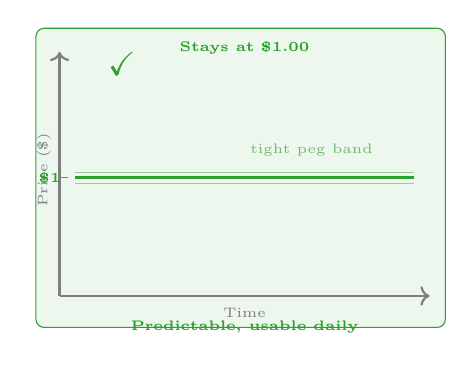
\begin{tikzpicture}
      % Chart background
      \draw[fill=mlgreen!8, draw=mlgreen, rounded corners=3pt] (0,0) rectangle (5.2,3.8);
      % Axes
      \draw[->, mlgray, thick] (0.3,0.4) -- (5.0,0.4);
      \draw[->, mlgray, thick] (0.3,0.4) -- (0.3,3.5);
      \node[font=\tiny, mlgray, rotate=90] at (0.1,2.0) {Price (\$)};
      \node[font=\tiny, mlgray] at (2.65,0.18) {Time};
      % Flat \$1 line
      \draw[mlgreen, very thick] (0.5,1.9) -- (4.8,1.9);
      % \$1 label
      \node[font=\tiny\bfseries, mlgreen] at (0.18,1.9) {\$1};
      \draw[mlgray, dashed, thin] (0.3,1.9) -- (0.5,1.9);
      % Minor band (peg band)
      \draw[mlgreen!50, thin] (0.5,1.97) -- (4.8,1.97);
      \draw[mlgreen!50, thin] (0.5,1.83) -- (4.8,1.83);
      \node[font=\tiny, mlgreen!70, align=center] at (3.5,2.25) {tight peg band};
      % Labels
      \node[font=\tiny\bfseries, mlgreen, align=center] at (2.65,3.55) {Stays at \$1.00};
      % Happy checkmark
      \node[font=\large, mlgreen] at (1.1,3.35) {\checkmark};
      \node[font=\tiny\bfseries, mlgreen, align=center] at (2.65,0.0) {Predictable, usable daily};
    \end{tikzpicture}
  \end{column}
\end{columns}

\bottomnote{A stablecoin maintains a fixed value (peg) --- usually \$1 --- by design, making it usable for real payments.}
\end{frame}

% ==================== FRAME 4: TYPES OF STABLECOINS ====================
\begin{frame}{Types of Stablecoins}
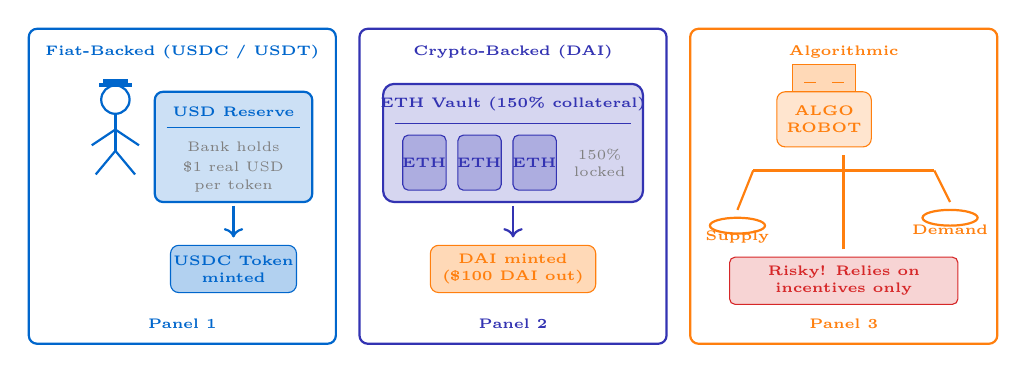
\begin{tikzpicture}
  % Panel borders
  \draw[thick, mlblue,   rounded corners=3pt] (0.1,0.2) rectangle (4.0,4.2);
  \draw[thick, mlpurple, rounded corners=3pt] (4.3,0.2) rectangle (8.2,4.2);
  \draw[thick, mlorange, rounded corners=3pt] (8.5,0.2) rectangle (12.4,4.2);

  % --- Panel 1: Fiat-backed ---
  \node[font=\tiny\bfseries, mlblue] at (2.05,3.9) {Fiat-Backed (USDC / USDT)};
  % Banker stick figure
  \draw[mlblue,thick] (1.2,3.3) circle (0.18);
  \draw[mlblue,thick] (1.2,3.12) -- (1.2,2.65);
  \draw[mlblue,thick] (1.2,2.92) -- (0.9,2.72);
  \draw[mlblue,thick] (1.2,2.92) -- (1.5,2.72);
  \draw[mlblue,thick] (1.2,2.65) -- (0.95,2.35);
  \draw[mlblue,thick] (1.2,2.65) -- (1.45,2.35);
  % Hat for banker
  \draw[fill=mlblue, draw=mlblue] (1.05,3.48) rectangle (1.35,3.55);
  \draw[fill=mlblue, draw=mlblue] (1.0,3.47) rectangle (1.4,3.5);
  % USD reserve vault
  \draw[fill=mlblue!20, draw=mlblue, thick, rounded corners=3pt]
       (1.7,2.0) rectangle (3.7,3.4);
  \node[font=\tiny\bfseries, mlblue, align=center] at (2.7,3.15) {USD Reserve};
  \draw[mlblue, thin] (1.85,2.95) -- (3.55,2.95);
  \node[font=\tiny, mlgray, align=center] at (2.7,2.7) {Bank holds};
  \node[font=\tiny, mlgray, align=center] at (2.7,2.45) {\$1 real USD};
  \node[font=\tiny, mlgray, align=center] at (2.7,2.2) {per token};
  % Minting arrow
  \draw[->, mlblue, thick] (2.7,1.95) -- (2.7,1.55);
  % USDC token
  \draw[fill=mlblue!30, draw=mlblue, rounded corners=3pt] (1.9,0.85) rectangle (3.5,1.45);
  \node[font=\tiny\bfseries, mlblue, align=center] at (2.7,1.15) {USDC Token\\minted};
  \node[font=\tiny\bfseries, mlblue] at (2.05,0.45) {Panel 1};

  % --- Panel 2: Crypto-backed (DAI) ---
  \node[font=\tiny\bfseries, mlpurple] at (6.25,3.9) {Crypto-Backed (DAI)};
  % Vault box overflowing with ETH
  \draw[fill=mlpurple!20, draw=mlpurple, thick, rounded corners=4pt]
       (4.6,2.0) rectangle (7.9,3.5);
  \node[font=\tiny\bfseries, mlpurple, align=center] at (6.25,3.25) {ETH Vault (150\% collateral)};
  \draw[mlpurple, thin] (4.75,3.0) -- (7.75,3.0);
  % ETH icons inside vault
  \draw[fill=mlpurple!40, draw=mlpurple, rounded corners=2pt] (4.85,2.15) rectangle (5.4,2.85);
  \node[font=\tiny\bfseries, mlpurple, align=center] at (5.12,2.5) {ETH};
  \draw[fill=mlpurple!40, draw=mlpurple, rounded corners=2pt] (5.55,2.15) rectangle (6.1,2.85);
  \node[font=\tiny\bfseries, mlpurple, align=center] at (5.82,2.5) {ETH};
  \draw[fill=mlpurple!40, draw=mlpurple, rounded corners=2pt] (6.25,2.15) rectangle (6.8,2.85);
  \node[font=\tiny\bfseries, mlpurple, align=center] at (6.52,2.5) {ETH};
  \node[font=\tiny, mlgray, align=center] at (7.35,2.5) {150\%\\locked};
  % Down arrow: smaller DAI comes out
  \draw[->, mlpurple, thick] (6.25,1.95) -- (6.25,1.55);
  % DAI token
  \draw[fill=mlorange!30, draw=mlorange, rounded corners=3pt] (5.2,0.85) rectangle (7.3,1.45);
  \node[font=\tiny\bfseries, mlorange, align=center] at (6.25,1.15) {DAI minted\\(\$100 DAI out)};
  \node[font=\tiny\bfseries, mlpurple] at (6.25,0.45) {Panel 2};

  % --- Panel 3: Algorithmic ---
  \node[font=\tiny\bfseries, mlorange] at (10.45,3.9) {Algorithmic};
  % Robot body
  \draw[fill=mlorange!20, draw=mlorange, rounded corners=3pt] (9.6,2.7) rectangle (10.8,3.4);
  \node[font=\tiny\bfseries, mlorange, align=center] at (10.2,3.05) {ALGO\\ROBOT};
  % Robot head
  \draw[fill=mlorange!30, draw=mlorange] (9.8,3.4) rectangle (10.6,3.75);
  \draw[mlorange, thin] (9.95,3.52) -- (10.1,3.52);
  \draw[mlorange, thin] (10.3,3.52) -- (10.45,3.52);
  % Balance scales
  % Scale pole
  \draw[mlorange, very thick] (10.45,1.4) -- (10.45,2.6);
  % Scale beam
  \draw[mlorange, very thick] (9.3,2.4) -- (11.6,2.4);
  % Left pan (supply)
  \draw[mlorange, thick] (9.3,2.4) -- (9.1,1.9);
  \draw[mlorange, thick] (9.1,1.7) ellipse (0.35 and 0.1);
  \node[font=\tiny\bfseries, mlorange, align=center] at (9.1,1.55) {Supply};
  % Right pan (demand) -- tilted
  \draw[mlorange, thick] (11.6,2.4) -- (11.8,2.0);
  \draw[mlorange, thick] (11.8,1.8) ellipse (0.35 and 0.1);
  \node[font=\tiny\bfseries, mlorange, align=center] at (11.8,1.65) {Demand};
  % Wobble label
  \draw[fill=mlred!20, draw=mlred, rounded corners=2pt] (9.0,0.7) rectangle (11.9,1.3);
  \node[font=\tiny\bfseries, mlred, align=center] at (10.45,1.0) {Risky! Relies on\\incentives only};
  \node[font=\tiny\bfseries, mlorange] at (10.45,0.45) {Panel 3};
\end{tikzpicture}

\bottomnote{Three archetypes: fiat-backed (safest), crypto-backed (decentralized), algorithmic (highest risk).}
\end{frame}

% ==================== FRAME 5: HOW STABLECOINS MAINTAIN THEIR PEG ====================
\begin{frame}{How Stablecoins Maintain Their Peg}
\centering
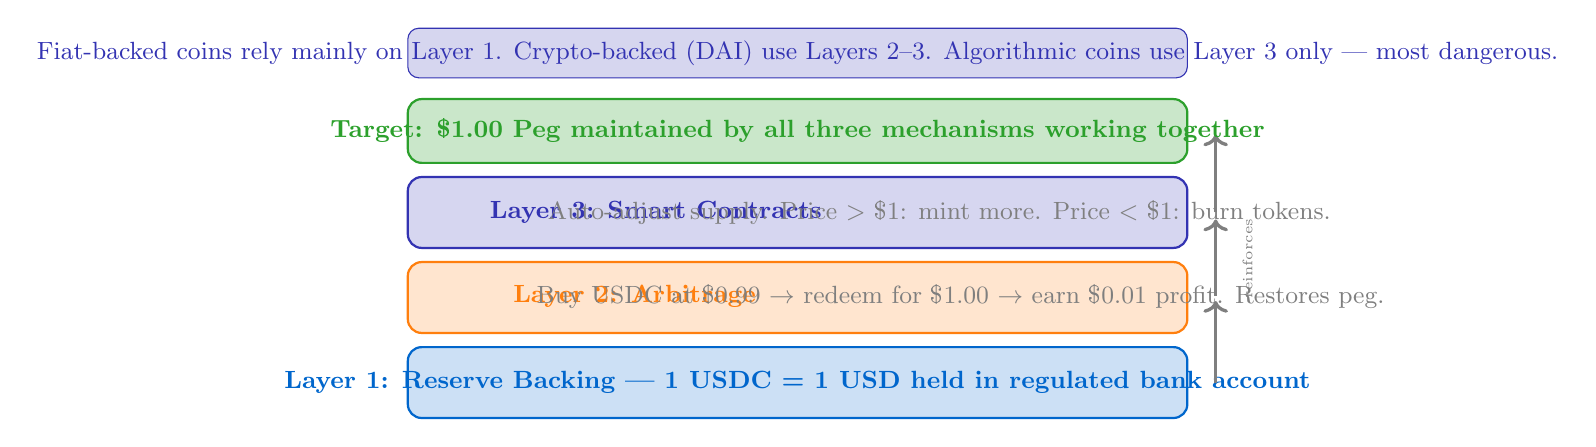
\begin{tikzpicture}[scale=0.90]
  % Layer 1 -- Reserve Backing (bottom)
  \draw[fill=mlblue!20, draw=mlblue, rounded corners=5pt, thick]
       (0,0) rectangle (11,1.0);
  \node[font=\small\bfseries, mlblue, align=center] at (5.5,0.5)
       {Layer 1: Reserve Backing --- 1 USDC = 1 USD held in regulated bank account};

  % Arrow up
  \draw[->, very thick, mlgray] (11.4,0.5) -- (11.4,1.65);

  % Layer 2 -- Arbitrage
  \draw[fill=mlorange!20, draw=mlorange, rounded corners=5pt, thick]
       (0,1.2) rectangle (11,2.2);
  \node[font=\small\bfseries, mlorange, align=center] at (3.2,1.72)
       {Layer 2: Arbitrage};
  \node[font=\small, mlgray, align=center] at (7.8,1.72)
       {Buy USDC at \$0.99 $\rightarrow$ redeem for \$1.00 $\rightarrow$ earn \$0.01 profit. Restores peg.};

  % Arrow up
  \draw[->, very thick, mlgray] (11.4,1.72) -- (11.4,2.8);

  % Layer 3 -- Smart Contract Logic
  \draw[fill=mlpurple!20, draw=mlpurple, rounded corners=5pt, thick]
       (0,2.4) rectangle (11,3.4);
  \node[font=\small\bfseries, mlpurple, align=center] at (3.5,2.9)
       {Layer 3: Smart Contracts};
  \node[font=\small, mlgray, align=center] at (7.5,2.9)
       {Auto-adjust supply. Price $>$ \$1: mint more. Price $<$ \$1: burn tokens.};

  % Arrow up
  \draw[->, very thick, mlgray] (11.4,2.9) -- (11.4,4.0);

  % Peg target at top
  \draw[fill=mlgreen!25, draw=mlgreen, rounded corners=5pt, thick]
       (0,3.6) rectangle (11,4.5);
  \node[font=\small\bfseries, mlgreen, align=center] at (5.5,4.05)
       {Target: \$1.00 Peg maintained by all three mechanisms working together};

  % Side label
  \node[font=\tiny, mlgray, rotate=90] at (11.85,2.25) {reinforces};

  % Summary info box below
  \draw[fill=mllavender4, draw=mlpurple, rounded corners=4pt] (0,4.8) rectangle (11,5.5);
  \node[font=\small, mlpurple, align=center] at (5.5,5.15)
       {Fiat-backed coins rely mainly on Layer 1.
        Crypto-backed (DAI) use Layers 2--3.
        Algorithmic coins use Layer 3 only --- most dangerous.};
\end{tikzpicture}

\bottomnote{Peg stability requires at least one reliable mechanism; relying solely on algorithmic incentives has repeatedly failed.}
\end{frame}

% ==================== FRAME 6: THE TERRA/LUNA DISASTER ====================
\begin{frame}{The Terra/LUNA Disaster (May 2022)}
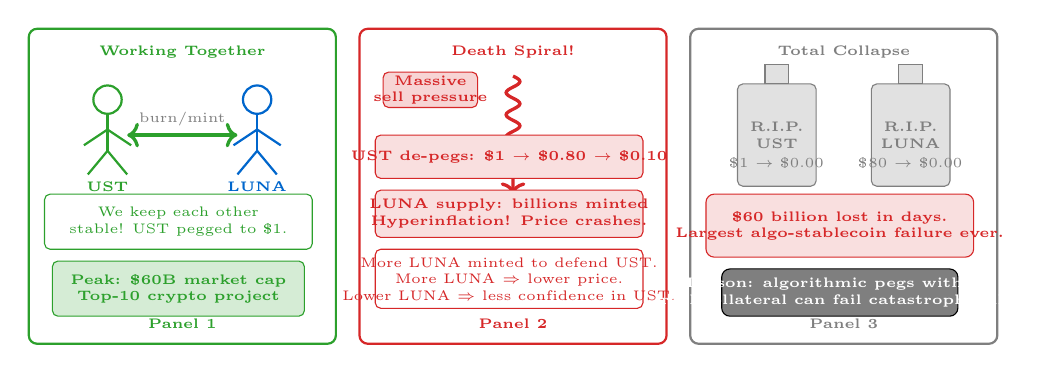
\begin{tikzpicture}
  % Panel borders
  \draw[thick, mlgreen,  rounded corners=3pt] (0.1,0.2) rectangle (4.0,4.2);
  \draw[thick, mlred,    rounded corners=3pt] (4.3,0.2) rectangle (8.2,4.2);
  \draw[thick, mlgray,   rounded corners=3pt] (8.5,0.2) rectangle (12.4,4.2);

  % --- Panel 1: UST and LUNA working together happily ---
  \node[font=\tiny\bfseries, mlgreen] at (2.05,3.9) {Working Together};
  % UST figure (green)
  \draw[mlgreen,thick] (1.1,3.3) circle (0.18);
  \draw[mlgreen,thick] (1.1,3.12) -- (1.1,2.65);
  \draw[mlgreen,thick] (1.1,2.92) -- (0.8,2.72);
  \draw[mlgreen,thick] (1.1,2.92) -- (1.4,2.72);
  \draw[mlgreen,thick] (1.1,2.65) -- (0.85,2.35);
  \draw[mlgreen,thick] (1.1,2.65) -- (1.35,2.35);
  \node[font=\tiny\bfseries, mlgreen] at (1.1,2.2) {UST};
  % LUNA figure (blue)
  \draw[mlblue,thick] (3.0,3.3) circle (0.18);
  \draw[mlblue,thick] (3.0,3.12) -- (3.0,2.65);
  \draw[mlblue,thick] (3.0,2.92) -- (2.7,2.72);
  \draw[mlblue,thick] (3.0,2.92) -- (3.3,2.72);
  \draw[mlblue,thick] (3.0,2.65) -- (2.75,2.35);
  \draw[mlblue,thick] (3.0,2.65) -- (3.25,2.35);
  \node[font=\tiny\bfseries, mlblue] at (3.0,2.2) {LUNA};
  % Double-headed arrow between them
  \draw[<->, very thick, mlgreen] (1.35,2.85) -- (2.75,2.85);
  \node[font=\tiny, mlgray, align=center] at (2.05,3.05) {burn/mint};
  % Speech bubble
  \draw[fill=white, draw=mlgreen, rounded corners=2pt] (0.3,1.4) rectangle (3.7,2.1);
  \node[font=\tiny, mlgreen, align=center] at (2.0,1.75) {We keep each other\\stable! UST pegged to \$1.};
  % Market cap box
  \draw[fill=mlgreen!20, draw=mlgreen, rounded corners=2pt] (0.4,0.55) rectangle (3.6,1.25);
  \node[font=\tiny\bfseries, mlgreen, align=center] at (2.0,0.9) {Peak: \$60B market cap\\Top-10 crypto project};
  \node[font=\tiny\bfseries, mlgreen] at (2.05,0.45) {Panel 1};

  % --- Panel 2: Death spiral ---
  \node[font=\tiny\bfseries, mlred] at (6.25,3.9) {Death Spiral!};
  % Down spiral arrow
  \draw[->, mlred, very thick, decoration={coil, aspect=0, segment length=8pt}, decorate]
       (6.25,3.6) -- (6.25,2.1);
  % Sell pressure label
  \draw[fill=mlred!20, draw=mlred, rounded corners=2pt] (4.6,3.2) rectangle (5.8,3.65);
  \node[font=\tiny\bfseries, mlred, align=center] at (5.2,3.42) {Massive\\sell pressure};
  % UST de-pegs
  \draw[fill=mlred!15, draw=mlred, rounded corners=2pt] (4.5,2.3) rectangle (7.9,2.85);
  \node[font=\tiny\bfseries, mlred, align=center] at (6.2,2.57) {UST de-pegs: \$1 $\rightarrow$ \$0.80 $\rightarrow$ \$0.10};
  % LUNA supply explodes
  \draw[fill=mlred!15, draw=mlred, rounded corners=2pt] (4.5,1.55) rectangle (7.9,2.15);
  \node[font=\tiny\bfseries, mlred, align=center] at (6.2,1.85) {LUNA supply: billions minted\\Hyperinflation! Price crashes.};
  % Speech bubble panic
  \draw[fill=white, draw=mlred, rounded corners=2pt] (4.5,0.65) rectangle (7.9,1.4);
  \node[font=\tiny, mlred, align=center] at (6.2,1.02) {More LUNA minted to defend UST.\\More LUNA $\Rightarrow$ lower price.\\Lower LUNA $\Rightarrow$ less confidence in UST.};
  \node[font=\tiny\bfseries, mlred] at (6.25,0.45) {Panel 2};

  % --- Panel 3: Collapse ---
  \node[font=\tiny\bfseries, mlgray] at (10.45,3.9) {Total Collapse};
  % Gravestone for UST
  \draw[fill=midgray!40, draw=mlgray, rounded corners=2pt] (9.1,2.2) rectangle (10.1,3.5);
  \draw[fill=midgray!40, draw=mlgray] (9.45,3.5) rectangle (9.75,3.75);
  \node[font=\tiny\bfseries, mlgray, align=center] at (9.6,2.85) {R.I.P.\\UST};
  \node[font=\tiny, mlgray, align=center] at (9.6,2.5) {\$1 $\rightarrow$ \$0.00};
  % Gravestone for LUNA
  \draw[fill=midgray!40, draw=mlgray, rounded corners=2pt] (10.8,2.2) rectangle (11.8,3.5);
  \draw[fill=midgray!40, draw=mlgray] (11.15,3.5) rectangle (11.45,3.75);
  \node[font=\tiny\bfseries, mlgray, align=center] at (11.3,2.85) {R.I.P.\\LUNA};
  \node[font=\tiny, mlgray, align=center] at (11.3,2.5) {\$80 $\rightarrow$ \$0.00};
  % Lesson box
  \draw[fill=mlred!15, draw=mlred, rounded corners=3pt] (8.7,1.3) rectangle (12.1,2.1);
  \node[font=\tiny\bfseries, mlred, align=center] at (10.4,1.7) {\$60 billion lost in days.\\Largest algo-stablecoin failure ever.};
  % Warning badge
  \draw[fill=mlgray, rounded corners=3pt] (8.9,0.55) rectangle (11.9,1.15);
  \node[font=\tiny\bfseries, white, align=center] at (10.4,0.85) {Lesson: algorithmic pegs without\\real collateral can fail catastrophically.};
  \node[font=\tiny\bfseries, mlgray] at (10.45,0.45) {Panel 3};
\end{tikzpicture}

\bottomnote{Terra/LUNA (May 2022): \$60B wiped out in days. The death spiral showed that algorithmic pegs without real backing are fragile.}
\end{frame}

% ==================== FRAME 7: WHAT IS A CBDC? ====================
\begin{frame}{What is a CBDC?}
\centering
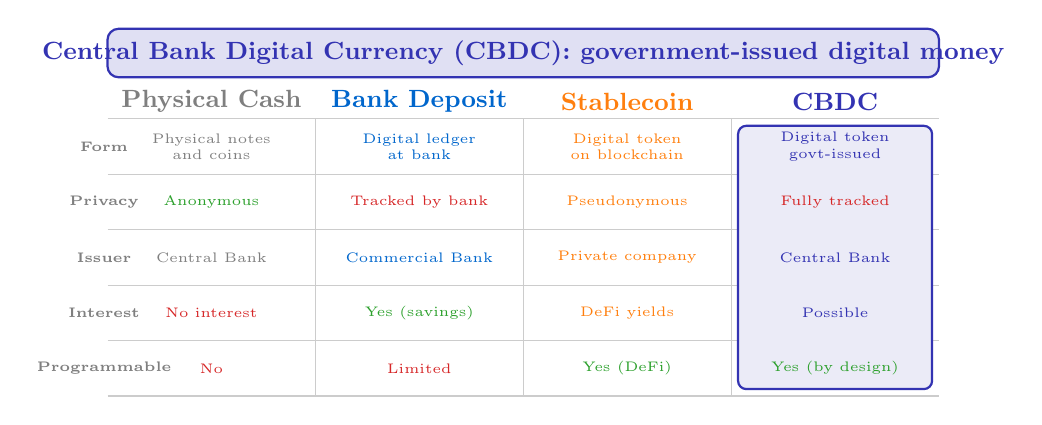
\begin{tikzpicture}[scale=0.88]
  % Header
  \draw[fill=mlpurple!15, draw=mlpurple, rounded corners=4pt, thick]
       (0,4.9) rectangle (12.0,5.6);
  \node[font=\small\bfseries, mlpurple, align=center] at (6.0,5.25)
       {Central Bank Digital Currency (CBDC): government-issued digital money};

  % Column headers
  \node[font=\small\bfseries, mlgray]    at (1.5,4.55)  {Physical Cash};
  \node[font=\small\bfseries, mlblue]    at (4.5,4.55)  {Bank Deposit};
  \node[font=\small\bfseries, mlorange]  at (7.5,4.55)  {Stablecoin};
  \node[font=\small\bfseries, mlpurple]  at (10.5,4.55) {CBDC};

  % Row labels
  \node[font=\tiny\bfseries, mlgray, align=right] at (-0.05,3.9) {Form};
  \node[font=\tiny\bfseries, mlgray, align=right] at (-0.05,3.1) {Privacy};
  \node[font=\tiny\bfseries, mlgray, align=right] at (-0.05,2.3) {Issuer};
  \node[font=\tiny\bfseries, mlgray, align=right] at (-0.05,1.5) {Interest};
  \node[font=\tiny\bfseries, mlgray, align=right] at (-0.05,0.7) {Programmable};

  % Divider lines
  \draw[mlgray!40, thin] (0,4.3) -- (12.0,4.3);
  \draw[mlgray!40, thin] (0,3.5) -- (12.0,3.5);
  \draw[mlgray!40, thin] (0,2.7) -- (12.0,2.7);
  \draw[mlgray!40, thin] (0,1.9) -- (12.0,1.9);
  \draw[mlgray!40, thin] (0,1.1) -- (12.0,1.1);
  \draw[mlgray!40, thin] (0,0.3) -- (12.0,0.3);
  \draw[mlgray!40, thin] (3.0,0.3) -- (3.0,4.3);
  \draw[mlgray!40, thin] (6.0,0.3) -- (6.0,4.3);
  \draw[mlgray!40, thin] (9.0,0.3) -- (9.0,4.3);

  % Physical Cash column
  \node[font=\tiny, mlgray, align=center] at (1.5,3.9) {Physical notes\\and coins};
  \node[font=\tiny, mlgreen, align=center] at (1.5,3.1) {Anonymous};
  \node[font=\tiny, mlgray, align=center]  at (1.5,2.3) {Central Bank};
  \node[font=\tiny, mlred, align=center]   at (1.5,1.5) {No interest};
  \node[font=\tiny, mlred, align=center]   at (1.5,0.7) {No};

  % Bank Deposit column
  \node[font=\tiny, mlblue, align=center]  at (4.5,3.9) {Digital ledger\\at bank};
  \node[font=\tiny, mlred, align=center]   at (4.5,3.1) {Tracked by bank};
  \node[font=\tiny, mlblue, align=center]  at (4.5,2.3) {Commercial Bank};
  \node[font=\tiny, mlgreen, align=center] at (4.5,1.5) {Yes (savings)};
  \node[font=\tiny, mlred, align=center]   at (4.5,0.7) {Limited};

  % Stablecoin column
  \node[font=\tiny, mlorange, align=center] at (7.5,3.9) {Digital token\\on blockchain};
  \node[font=\tiny, mlorange, align=center] at (7.5,3.1) {Pseudonymous};
  \node[font=\tiny, mlorange, align=center] at (7.5,2.3) {Private company};
  \node[font=\tiny, mlorange, align=center] at (7.5,1.5) {DeFi yields};
  \node[font=\tiny, mlgreen, align=center]  at (7.5,0.7) {Yes (DeFi)};

  % CBDC column (highlighted)
  \draw[fill=mlpurple!10, draw=mlpurple, thick, rounded corners=3pt]
       (9.1,0.4) rectangle (11.9,4.2);
  \node[font=\tiny, mlpurple, align=center] at (10.5,3.9) {Digital token\\govt-issued};
  \node[font=\tiny, mlred, align=center]    at (10.5,3.1) {Fully tracked};
  \node[font=\tiny, mlpurple, align=center] at (10.5,2.3) {Central Bank};
  \node[font=\tiny, mlpurple, align=center] at (10.5,1.5) {Possible};
  \node[font=\tiny, mlgreen, align=center]  at (10.5,0.7) {Yes (by design)};
\end{tikzpicture}

\bottomnote{A CBDC combines the legal tender status of cash with the programmability of crypto --- issued directly by the central bank.}
\end{frame}

% ==================== FRAME 8: CBDCs AROUND THE WORLD ====================
\begin{frame}{CBDCs Around the World}
\centering
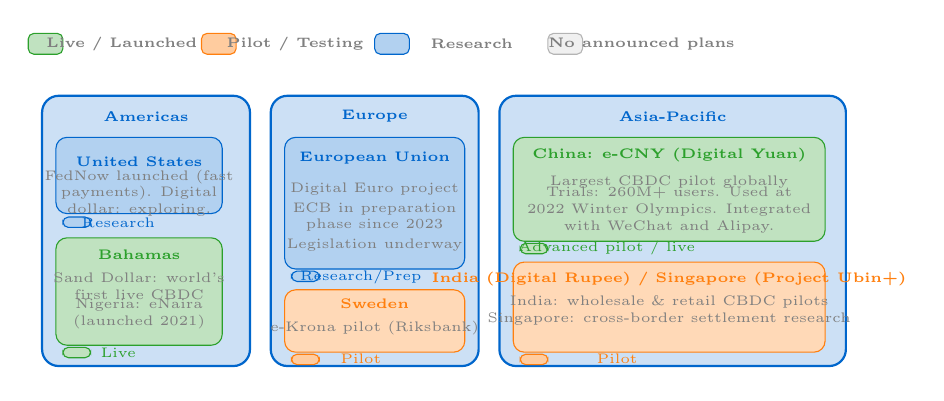
\begin{tikzpicture}[scale=0.88]
  % Legend
  \draw[fill=mlgreen!30,  draw=mlgreen,  rounded corners=2pt] (0.0,5.1) rectangle (0.5,5.4);
  \node[font=\tiny\bfseries, mlgray] at (1.35,5.25) {Live / Launched};
  \draw[fill=mlorange!40, draw=mlorange, rounded corners=2pt] (2.5,5.1) rectangle (3.0,5.4);
  \node[font=\tiny\bfseries, mlgray] at (3.85,5.25) {Pilot / Testing};
  \draw[fill=mlblue!30,   draw=mlblue,   rounded corners=2pt] (5.0,5.1) rectangle (5.5,5.4);
  \node[font=\tiny\bfseries, mlgray] at (6.4,5.25) {Research};
  \draw[fill=lightgray,   draw=midgray,  rounded corners=2pt] (7.5,5.1) rectangle (8.0,5.4);
  \node[font=\tiny\bfseries, mlgray] at (8.85,5.25) {No announced plans};

  % Simple stylized world map regions as rectangles/ellipses
  % Americas
  \draw[fill=mlblue!20, draw=mlblue, rounded corners=6pt, thick]
       (0.2,0.6) rectangle (3.2,4.5);
  \node[font=\tiny\bfseries, mlblue, align=center] at (1.7,4.2) {Americas};

  % USA
  \draw[fill=mlblue!30, draw=mlblue, rounded corners=4pt]
       (0.4,2.8) rectangle (2.8,3.9);
  \node[font=\tiny\bfseries, mlblue, align=center] at (1.6,3.55) {United States};
  \node[font=\tiny, mlgray, align=center] at (1.6,3.1) {FedNow launched (fast\\payments). Digital\\dollar: exploring.};
  \draw[fill=mlblue!30, draw=mlblue, rounded corners=2pt] (0.5,2.6) rectangle (0.9,2.75);
  \node[font=\tiny, mlblue] at (1.3,2.67) {Research};

  % Caribbean / Bahamas
  \draw[fill=mlgreen!30, draw=mlgreen, rounded corners=4pt]
       (0.4,0.9) rectangle (2.8,2.45);
  \node[font=\tiny\bfseries, mlgreen, align=center] at (1.6,2.2) {Bahamas};
  \node[font=\tiny, mlgray, align=center] at (1.6,1.75) {Sand Dollar: world's\\first live CBDC};
  \node[font=\tiny, mlgray, align=center] at (1.6,1.35) {Nigeria: eNaira\\(launched 2021)};
  \draw[fill=mlgreen!30, draw=mlgreen, rounded corners=2pt] (0.5,0.72) rectangle (0.9,0.87);
  \node[font=\tiny, mlgreen] at (1.3,0.79) {Live};

  % Europe
  \draw[fill=mlblue!20, draw=mlblue, rounded corners=6pt, thick]
       (3.5,0.6) rectangle (6.5,4.5);
  \node[font=\tiny\bfseries, mlblue, align=center] at (5.0,4.2) {Europe};

  % EU Digital Euro
  \draw[fill=mlblue!30, draw=mlblue, rounded corners=4pt]
       (3.7,2.0) rectangle (6.3,3.9);
  \node[font=\tiny\bfseries, mlblue, align=center] at (5.0,3.6) {European Union};
  \node[font=\tiny, mlgray, align=center] at (5.0,3.15) {Digital Euro project};
  \node[font=\tiny, mlgray, align=center] at (5.0,2.75) {ECB in preparation\\phase since 2023};
  \node[font=\tiny, mlgray, align=center] at (5.0,2.35) {Legislation underway};
  \draw[fill=mlblue!30, draw=mlblue, rounded corners=2pt] (3.8,1.82) rectangle (4.2,1.97);
  \node[font=\tiny, mlblue] at (4.8,1.89) {Research/Prep};

  % Sweden
  \draw[fill=mlorange!30, draw=mlorange, rounded corners=4pt]
       (3.7,0.8) rectangle (6.3,1.7);
  \node[font=\tiny\bfseries, mlorange, align=center] at (5.0,1.5) {Sweden};
  \node[font=\tiny, mlgray, align=center] at (5.0,1.15) {e-Krona pilot (Riksbank)};
  \draw[fill=mlorange!40, draw=mlorange, rounded corners=2pt] (3.8,0.62) rectangle (4.2,0.77);
  \node[font=\tiny, mlorange] at (4.8,0.7) {Pilot};

  % Asia-Pacific
  \draw[fill=mlblue!20, draw=mlblue, rounded corners=6pt, thick]
       (6.8,0.6) rectangle (11.8,4.5);
  \node[font=\tiny\bfseries, mlblue, align=center] at (9.3,4.2) {Asia-Pacific};

  % China e-CNY
  \draw[fill=mlgreen!30, draw=mlgreen, rounded corners=4pt]
       (7.0,2.4) rectangle (11.5,3.9);
  \node[font=\tiny\bfseries, mlgreen, align=center] at (9.25,3.65) {China: e-CNY (Digital Yuan)};
  \node[font=\tiny, mlgray, align=center] at (9.25,3.25) {Largest CBDC pilot globally};
  \node[font=\tiny, mlgray, align=center] at (9.25,2.85) {Trials: 260M+ users. Used at\\2022 Winter Olympics. Integrated\\with WeChat and Alipay.};
  \draw[fill=mlgreen!30, draw=mlgreen, rounded corners=2pt] (7.1,2.22) rectangle (7.5,2.37);
  \node[font=\tiny, mlgreen] at (8.35,2.3) {Advanced pilot / live};

  % India, Singapore, Australia
  \draw[fill=mlorange!30, draw=mlorange, rounded corners=4pt]
       (7.0,0.8) rectangle (11.5,2.1);
  \node[font=\tiny\bfseries, mlorange, align=center] at (9.25,1.85) {India (Digital Rupee) / Singapore (Project Ubin+)};
  \node[font=\tiny, mlgray, align=center] at (9.25,1.4) {India: wholesale \& retail CBDC pilots\\Singapore: cross-border settlement research};
  \draw[fill=mlorange!40, draw=mlorange, rounded corners=2pt] (7.1,0.62) rectangle (7.5,0.77);
  \node[font=\tiny, mlorange] at (8.5,0.7) {Pilot};
\end{tikzpicture}

\bottomnote{Over 130 countries are exploring CBDCs. China leads with the most advanced large-scale pilot; EU and US are in early stages.}
\end{frame}

% ==================== FRAME 9: RISKS AND BENEFITS ====================
\begin{frame}{Risks and Benefits of Stablecoins \& CBDCs}
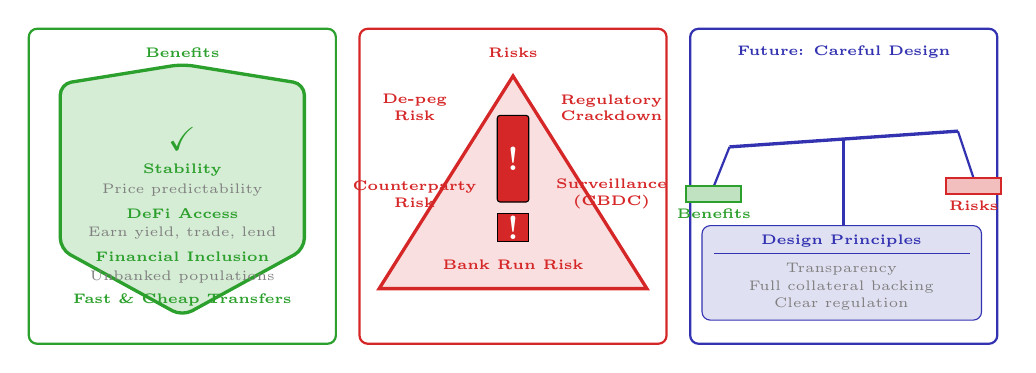
\begin{tikzpicture}
  % Panel borders
  \draw[thick, mlgreen,  rounded corners=3pt] (0.1,0.2) rectangle (4.0,4.2);
  \draw[thick, mlred,    rounded corners=3pt] (4.3,0.2) rectangle (8.2,4.2);
  \draw[thick, mlpurple, rounded corners=3pt] (8.5,0.2) rectangle (12.4,4.2);

  % --- Panel 1: Benefits shield ---
  \node[font=\tiny\bfseries, mlgreen] at (2.05,3.9) {Benefits};
  % Shield shape (polygon approximation)
  \draw[fill=mlgreen!20, draw=mlgreen, very thick, rounded corners=4pt]
       (0.5,1.4) -- (0.5,3.5) -- (2.05,3.75) -- (3.6,3.5) -- (3.6,1.4) --
       (2.05,0.55) -- cycle;
  % Shield star / check inside
  \node[font=\large\bfseries, mlgreen] at (2.05,2.8) {\checkmark};
  % Benefit items
  \node[font=\tiny\bfseries, mlgreen, align=center] at (2.05,2.4) {Stability};
  \node[font=\tiny, mlgray, align=center] at (2.05,2.15) {Price predictability};
  \node[font=\tiny\bfseries, mlgreen, align=center] at (2.05,1.85) {DeFi Access};
  \node[font=\tiny, mlgray, align=center] at (2.05,1.6) {Earn yield, trade, lend};
  \node[font=\tiny\bfseries, mlgreen, align=center] at (2.05,1.3) {Financial Inclusion};
  \node[font=\tiny, mlgray, align=center] at (2.05,1.05) {Unbanked populations};
  \node[font=\tiny\bfseries, mlgreen, align=center] at (2.05,0.75) {Fast \& Cheap Transfers};

  % --- Panel 2: Risks warning ---
  \node[font=\tiny\bfseries, mlred] at (6.25,3.9) {Risks};
  % Warning triangle (polygon)
  \draw[fill=mlred!15, draw=mlred, very thick]
       (6.25,3.6) -- (4.55,0.9) -- (7.95,0.9) -- cycle;
  % Exclamation mark inside
  \draw[fill=mlred, rounded corners=1pt] (6.05,2.0) rectangle (6.45,3.1);
  \draw[fill=mlred] (6.05,1.5) rectangle (6.45,1.85);
  \node[font=\large\bfseries, white] at (6.25,2.55) {!};
  \node[font=\large\bfseries, white] at (6.25,1.67) {!};
  % Risk labels outside triangle
  \node[font=\tiny\bfseries, mlred, align=center] at (5.0,3.2) {De-peg\\Risk};
  \node[font=\tiny\bfseries, mlred, align=center] at (7.5,3.2) {Regulatory\\Crackdown};
  \node[font=\tiny\bfseries, mlred, align=center] at (5.0,2.1) {Counterparty\\Risk};
  \node[font=\tiny\bfseries, mlred, align=center] at (7.5,2.1) {Surveillance\\(CBDC)};
  \node[font=\tiny\bfseries, mlred, align=center] at (6.25,1.2) {Bank Run Risk};

  % --- Panel 3: Balance scales for future ---
  \node[font=\tiny\bfseries, mlpurple] at (10.45,3.9) {Future: Careful Design};
  % Scale pole
  \draw[mlpurple, very thick] (10.45,1.2) -- (10.45,2.8);
  % Scale beam (slightly tilted toward benefits)
  \draw[mlpurple, very thick] (9.0,2.7) -- (11.9,2.9);
  % Left pan (benefits -- higher)
  \draw[mlpurple, thick] (9.0,2.7) -- (8.8,2.2);
  \draw[fill=mlgreen!30, draw=mlgreen, thick] (8.45,2.0) rectangle (9.15,2.2);
  \node[font=\tiny\bfseries, mlgreen, align=center] at (8.8,1.85) {Benefits};
  % Right pan (risks -- lower)
  \draw[mlpurple, thick] (11.9,2.9) -- (12.1,2.3);
  \draw[fill=mlred!30, draw=mlred, thick] (11.75,2.1) rectangle (12.45,2.3);
  \node[font=\tiny\bfseries, mlred, align=center] at (12.1,1.95) {Risks};
  % Design principles box
  \draw[fill=mlpurple!15, draw=mlpurple, rounded corners=3pt]
       (8.65,0.5) rectangle (12.2,1.7);
  \node[font=\tiny\bfseries, mlpurple, align=center] at (10.42,1.5) {Design Principles};
  \draw[mlpurple, thin] (8.8,1.35) -- (12.05,1.35);
  \node[font=\tiny, mlgray, align=center] at (10.42,1.15) {Transparency};
  \node[font=\tiny, mlgray, align=center] at (10.42,0.92) {Full collateral backing};
  \node[font=\tiny, mlgray, align=center] at (10.42,0.7) {Clear regulation};
\end{tikzpicture}

\bottomnote{The benefits of stablecoins are real, but so are the risks. Good design, collateral, and regulation determine survival.}
\end{frame}

% ==================== FRAME 10: KEY TAKEAWAYS ====================
\begin{frame}{Key Takeaways}
\centering
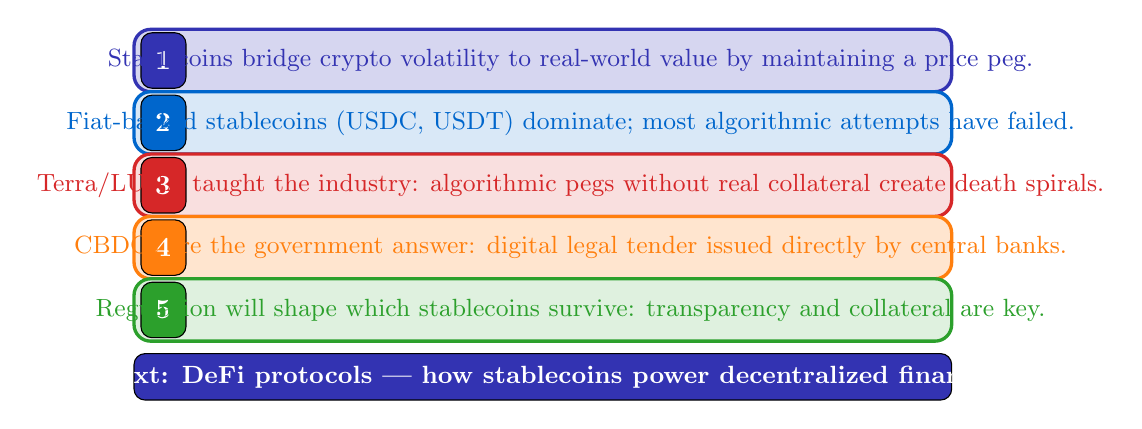
\begin{tikzpicture}[scale=0.88]
  % Box 1
  \draw[fill=mlpurple!20, draw=mlpurple, very thick, rounded corners=6pt]
       (0,4.0) rectangle (11.8,4.9);
  \draw[fill=mlpurple, rounded corners=4pt] (0.1,4.05) rectangle (0.75,4.85);
  \node[font=\normalsize\bfseries, white] at (0.42,4.45) {1};
  \node[font=\small, mlpurple, align=left] at (6.3,4.45)
       {Stablecoins bridge crypto volatility to real-world value by maintaining a price peg.};

  % Box 2
  \draw[fill=mlblue!15, draw=mlblue, very thick, rounded corners=6pt]
       (0,3.1) rectangle (11.8,4.0);
  \draw[fill=mlblue, rounded corners=4pt] (0.1,3.15) rectangle (0.75,3.95);
  \node[font=\normalsize\bfseries, white] at (0.42,3.55) {2};
  \node[font=\small, mlblue, align=left] at (6.3,3.55)
       {Fiat-backed stablecoins (USDC, USDT) dominate; most algorithmic attempts have failed.};

  % Box 3
  \draw[fill=mlred!15, draw=mlred, very thick, rounded corners=6pt]
       (0,2.2) rectangle (11.8,3.1);
  \draw[fill=mlred, rounded corners=4pt] (0.1,2.25) rectangle (0.75,3.05);
  \node[font=\normalsize\bfseries, white] at (0.42,2.65) {3};
  \node[font=\small, mlred, align=left] at (6.3,2.65)
       {Terra/LUNA taught the industry: algorithmic pegs without real collateral create death spirals.};

  % Box 4
  \draw[fill=mlorange!20, draw=mlorange, very thick, rounded corners=6pt]
       (0,1.3) rectangle (11.8,2.2);
  \draw[fill=mlorange, rounded corners=4pt] (0.1,1.35) rectangle (0.75,2.15);
  \node[font=\normalsize\bfseries, white] at (0.42,1.75) {4};
  \node[font=\small, mlorange, align=left] at (6.3,1.75)
       {CBDCs are the government answer: digital legal tender issued directly by central banks.};

  % Box 5
  \draw[fill=mlgreen!15, draw=mlgreen, very thick, rounded corners=6pt]
       (0,0.4) rectangle (11.8,1.3);
  \draw[fill=mlgreen, rounded corners=4pt] (0.1,0.45) rectangle (0.75,1.25);
  \node[font=\normalsize\bfseries, white] at (0.42,0.85) {5};
  \node[font=\small, mlgreen, align=left] at (6.3,0.85)
       {Regulation will shape which stablecoins survive: transparency and collateral are key.};

  % Purple teaser bar at bottom
  \draw[fill=mlpurple, rounded corners=4pt] (0,-0.45) rectangle (11.8,0.22);
  \node[font=\small\bfseries, white, align=center] at (5.9,-0.12)
       {Next: DeFi protocols --- how stablecoins power decentralized finance};
\end{tikzpicture}

\bottomnote{Stablecoins are the on-ramp to crypto's financial system. Understanding their mechanics and risks is essential for any practitioner.}
\end{frame}

\end{document}
